\begin{landscape}
\section{Statemachines (Kristian S. og David)}

\subsubsection{Statemachine over UART/transmitter }

\begin{figure}[h]
\centering
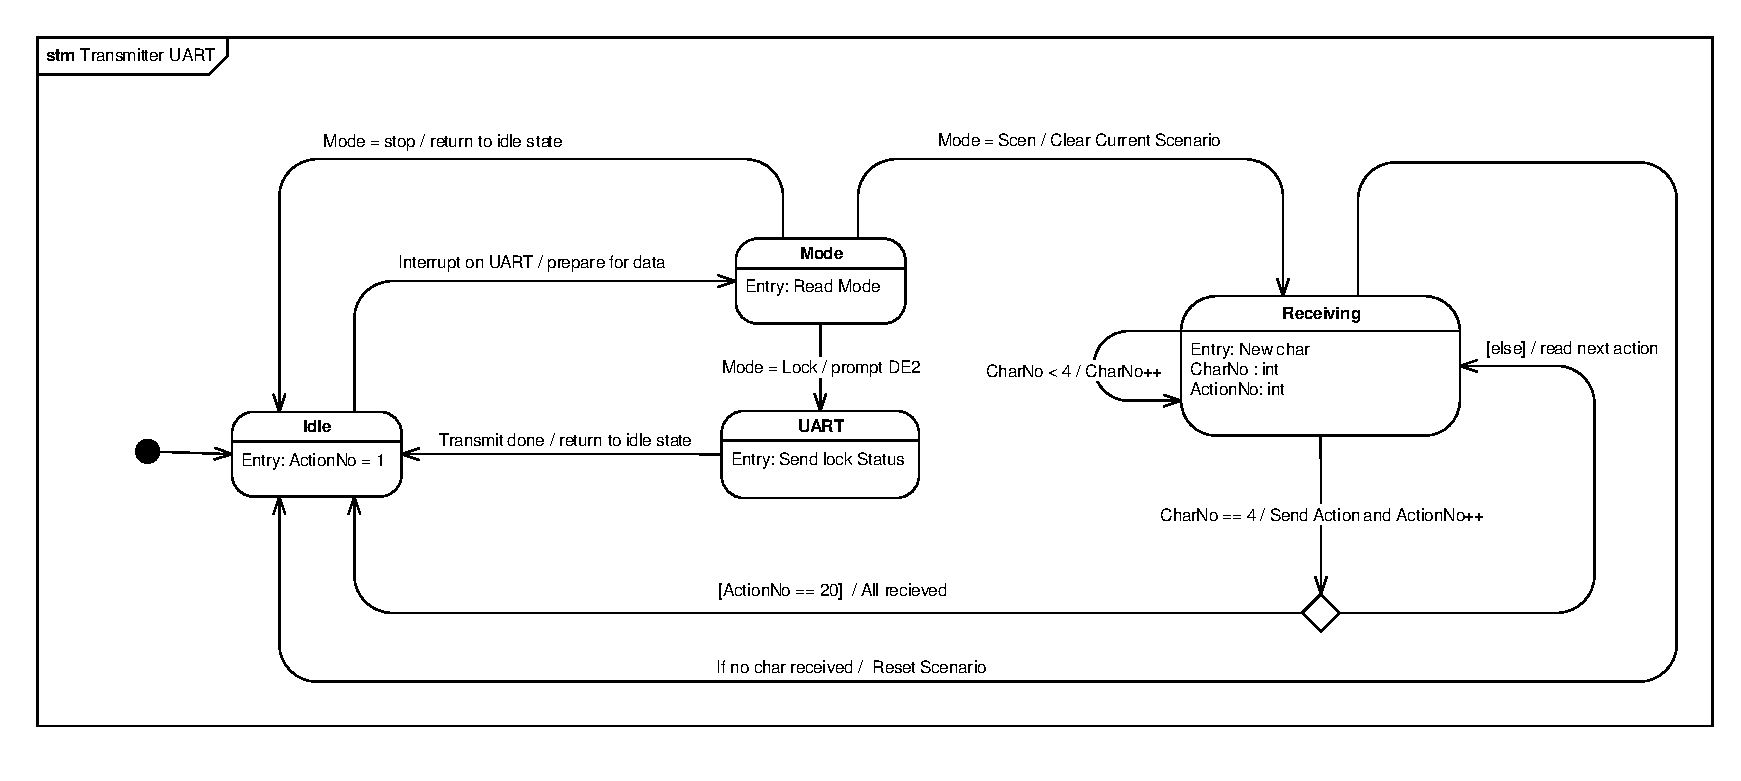
\includegraphics[width=\textheight + 190pt,clip=true, trim=18 18 10 18]{Systemarkitektur/diagrammer/Stm_transmitter_UART} %L B R T - HUSKE DET
\end{figure}

Statemachinen viser Transmitteren's tilstande når PC'en sender data over UART'en. Den første block Mode er et af følgende: Lock, Stop, og Scen(Scenarie). Hvis Scen er sendt, gør transmitter klar til at modtage flere data om det nye scenarie. Efter alt data er modtaget, starter transmitteren det nye scenariet og returner til idle tilstanden.

\newpage

\subsubsection{Statemachine over X.10/transmitter }

\begin{figure}[h]
\centering
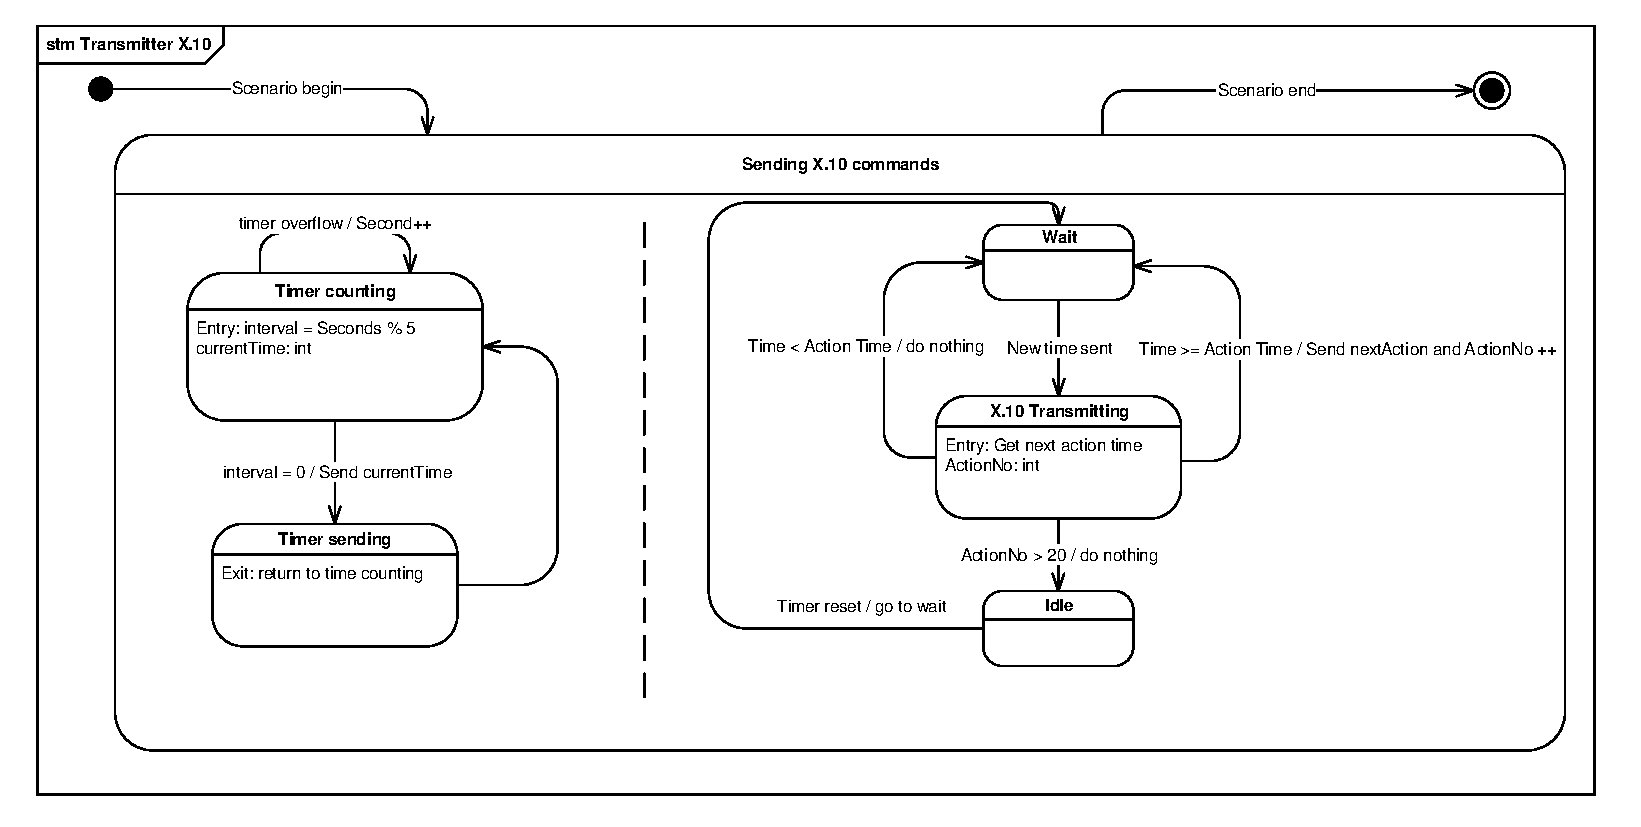
\includegraphics[width=\textheight + 190pt,clip=true, trim=18 15 18 12]{Systemarkitektur/diagrammer/Stm_transmitter_X10} %L B R T - HUSKE DET
\end{figure}

Denne statemachine viser det parallele forløb mellem Time, som holder styr på tiden, og transmitteren, der modtager tid fra Time, samt sender X.10 data ud til Tx10 Klassen.

\clearpage

\subsubsection{Statemachine over X.10/receiver}

\begin{figure}[h]
\centering
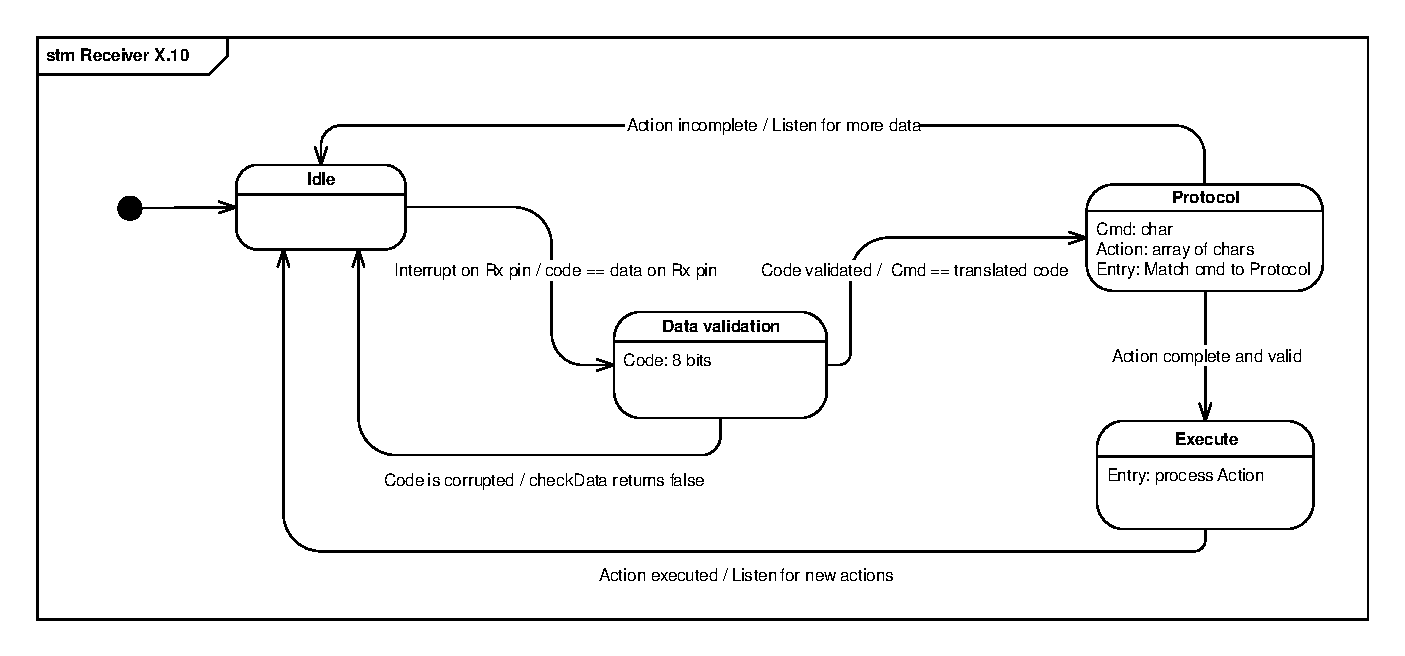
\includegraphics[width=\textheight + 190pt,clip=true, trim=18 15 15 12]{Systemarkitektur/diagrammer/Stm_receiver_X10}
\end{figure}

Her ses de forskellige tilstande receiveren skal gennemgå, når data modtages fra X.10 nettet. Når data modtages, loades de ind i en buffer, og checkes op mod X.10 protokollen. Hvis kommandoen er korrekt, vil den blive eksekveret, ellers skal den kastede kommandoen væk. Receiven lytter derefter for mere data. 



\end{landscape}

\clearpage